%% SECTION: CYCLES DE MILANKOVITCH

\paragraph{} Les variations du flux de chaleur solaire dans la théorie de Milankovitch sont dû à des cycles dans les paramètres de la trajectoire de la Terre. Les paramètres considérés par Milankovitch sont l'obliquité, l'excentricité et la précession axiale. L'obliquité $\varepsilon$ est l'angle entre l'axe de rotation Terrestre et la normale au plan orbital. L'excentricité $e$ est une mesure du caractère elliptique de la trajectoire et est reliée au grand et petit demi-axes de l'ellipse, respectivement $a$ et $b$, par la formule

\begin{equation}
	e = \sqrt{1-\frac{b^2}{a^2}}.
\end{equation}
Enfin, la précession axiale est la rotation de l'axe de rotation par rapport au repère fixe des étoiles. Le paramètre suivi dans le cas de la précession est le sinus de l'angle $\bar\omega$ décrivant l'état de l'axe dans sa rotation. La figure \ref{fig:MilankovitchCyclesOrbitandCores} reprend l'évolution de ces paramètres orbitaux sur environ 800\,kA avant et après l'instant présent.

\begin{figure}[t]
	\centering
	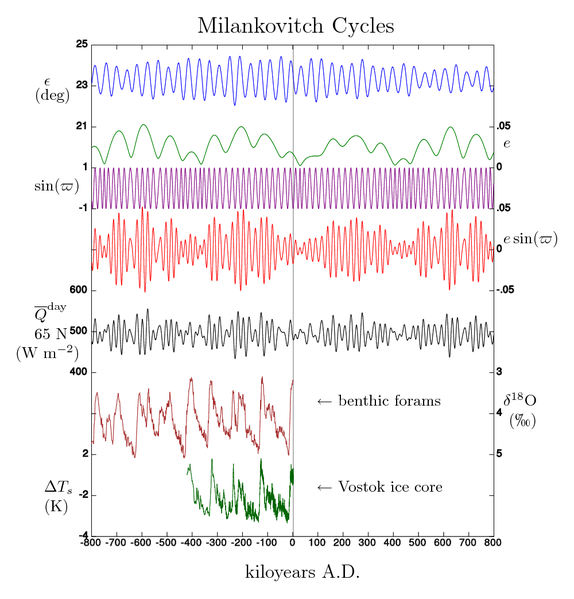
\includegraphics[width=0.9\linewidth]{figures/MilankovitchCyclesOrbitandCores}
	\caption{Cycles de Milankovitch: évolution des paramètres orbitaux. Image tirée de \cite{wiki_milankovitch_cycles}.}
	\label{fig:MilankovitchCyclesOrbitandCores}
\end{figure}

\paragraph{} Le cycle décrit par l'obliquité a une période principale de 41\,kA, i.e. principal pic dans la décomposition spectrale. Il est communément tenu pour responsable de la variation du climat durant le début du pléistocène (2.6\,MA à 0.9\,MA), période durant laquelle le rythme des glaciations suit le cycle d'obliquité de manière assez li
néaire \cite{huggett}. Le cycle décrit par l'excentricité a des pics à 95,125 et environ 400\,kA. Les deux premiers pics, se combinant à environ 100\,kA, sont des candidats pour expliquer l'écart de 100\,kA entre les glaciations plus récentes. Le cycle de précession se compose quant à lui de signaux de 19 et 23\,kA \cite{huggett} \cite{wiki_milankovitch_cycles}.

\paragraph{} Un autre cycle, écarté par Milankovitch pour ne pas avoir d'influence directe sur le flux solaire, est celui de l'inclinaison du plan orbital de la Terre par rapport au repère fixe des étoiles. Celui-ci a une période principale de 100\,kA et intervient ainsi dans certains modèles pour expliquer les dernières glaciations \cite{muller1995}.
